\documentclass[12pt]{article}

\usepackage[a4paper,margin=1in]{geometry}
\usepackage[utf8]{inputenc}
\usepackage{setspace}
\usepackage{amsmath}
\usepackage{amssymb}
\usepackage{listings}
\usepackage{xcolor}
\usepackage{graphicx}
\usepackage{float}
\usepackage{url} 
\usepackage{hyperref}
\usepackage[backend=biber,style=numeric]{biblatex}
\addbibresource{references.bib}
\usepackage{booktabs}
\usepackage{subcaption}
\usepackage{amsfonts} 
\def\sone{{\textbf{1}}}

\begin{document}

% --------- Title Page ---------
\begin{titlepage}
    \centering
    {\Huge \textbf{Assignment 1} \par}
    \vspace{1.5cm}
    {\Large \textbf{Advanced Machine Learning} \par}
    \vspace{2cm}
    {\large Mincu Adrian-Lucian \par} % <-- Replace with your name
    \vfill
    {\large May 2026 \par}
\end{titlepage}

% --------- Table of Contents ---------
\tableofcontents
\newpage

% --------- Solved Exercises ---------
\section*{Exercise 1}
\addcontentsline{toc}{section}{Exercise 1}

1. \textbf{(0.3 points)} What is the maximum value of the natural even number $n$, $n=2m$, such that there exists a hypothesis class $\mathcal{H}$ with $n$ elements that shatters a set C of $m = \frac{n}{2}$ points? Give an example of such an $\mathcal{H}$ and C. Justify your answer.
\newline

To shatter a set $C$ of size $m$, the hypothesis class $\mathcal{H}$ must be large enough to realize every possible case over $C$. This requires:
$$|\mathcal{H}| \geq 2^m$$
Given that $n = 2^m$, the condition becomes $2m \geq 2^m$ for $m \in \mathbb{N}^*$. Checking small values:

\noindent For $m = 1$: $2(1) \geq 2^1 \Rightarrow 2 \geq 2$ \quad \checkmark

\noindent For $m = 2$: $2(2) \geq 2^2 \Rightarrow 4 \geq 4$ \quad \checkmark

\noindent For $m = 3$: $2(3) \geq 2^3 \Rightarrow 6 \geq 8$ \quad \texttimes
\newline 

\noindent We claim $m = 2$ is the largest integer satisfying the inequality. Define:
$$g : [3, +\infty) \to \mathbb{R}, \qquad g(x) = 2x - 2^x$$
Computing the derivative gives:
$$g'(x) = 2 - 2^x \ln 2$$
Since $2^x \ln 2 > 2$ for all $x \geq 3$, we have $g'(x) < 0$ throughout $[3, +\infty)$, so $g$ is strictly decreasing on this interval. This means:
$$g(x) \leq g(3) = 6 - 8 = -2 < 0, \qquad \forall\, x \in [3, +\infty)$$
\noindent This confirms that $2m < 2^m$ holds for every integer $m \geq 3$, making $m = 2$ (or $n = 4$) the maximum valid value.
\newline

Take $C = \{x_1, x_2\}$ and define $\mathcal{H} = \{h_1, h_2, h_3, h_4\}$ via the following labeling table:

\begin{center}
\begin{tabular}{c|cc}
    & $x_1$ & $x_2$ \\
\hline
$h_1$ & $0$ & $0$ \\
$h_2$ & $1$ & $0$ \\
$h_3$ & $0$ & $1$ \\
$h_4$ & $1$ & $1$ \\
\end{tabular}
\end{center}

\noindent Every one of the $2^2 = 4$ distinct binary labelings of $C$ appears as a row, so $\mathcal{H}$ shatters $C$.

\newpage
\section*{Exercise 2}
\addcontentsline{toc}{section}{Exercise 2}

2. \textbf{(1.2 points)} Consider $\mathcal{H} = \mathcal{H}_1 \cup \mathcal{H}_2 \cup \mathcal{H}_3$, where:

\begin{itemize}
    \setlength{\itemindent}{-6mm}
    \item[] $\mathcal{H}_1 = \{h_{a} : \mathbb{R} \rightarrow \{0,1\} \ | \ h_{a}(x) = \sone_{[x \geq a]}(x) = \sone_{[a, +\infty)}(x), a \in \mathbb{R}\}$,
    \item[] $\mathcal{H}_2 = \{h_{a} : \mathbb{R} \rightarrow \{0,1\} \ | \ h_{a}(x) = \sone_{[x < a]}(x) = \sone_{(-\infty, a)}(x), a \in \mathbb{R}\}$,
    \item[] $\mathcal{H}_3 = \{h_{a, b} : \mathbb{R} \rightarrow \{0,1\} \ | \ h_{a, b}(x) = \sone_{[a \leq x \leq b]}(x) = \sone_{[a, b]}(x), a, b \in \mathbb{R}\}$.
\end{itemize}    

Consider the realizability assumption.

\begin{itemize}
    \item[a)] Compute VCdim($\mathcal{H}$).
    \item[b)] Give an algorithm A and determine an upper bound on the sample complexity $m_{\mathcal{H}}(\epsilon, \delta)$ such that the definition of PAC-learnability is satisfied.
    
\end{itemize}

\subsection*{(a)}
\addcontentsline{toc}{subsection}{(a)}

\begin{figure}[H]
\centering
\begin{subfigure}{0.32\textwidth}
    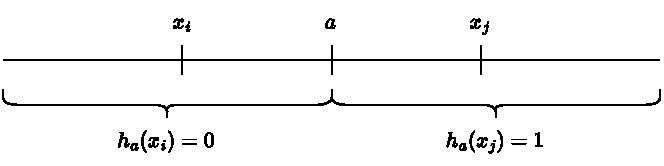
\includegraphics[width=\textwidth]{figures/2a_fig1.pdf}
    \caption{}
    \label{fig:2a_fig1}
\end{subfigure}
\hfill
\begin{subfigure}{0.32\textwidth}
    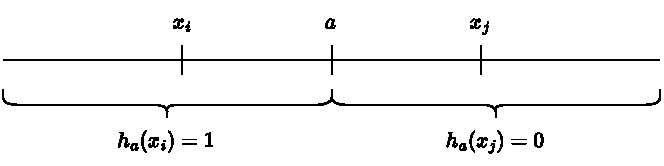
\includegraphics[width=\textwidth]{figures/2a_fig2.pdf}
    \caption{}
    \label{fig:2a_fig2}
\end{subfigure}
\hfill
\begin{subfigure}{0.32\textwidth}
    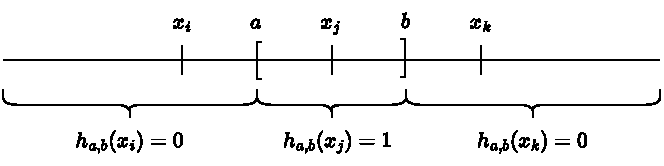
\includegraphics[width=\textwidth]{figures/2a_fig3.pdf}
    \caption{}
    \label{fig:2a_fig3}
\end{subfigure}
\caption{}
\end{figure}

\noindent We will compute the $\mathrm{VCdim}$ for each hypothesis class.
\newline

\noindent\textbf{$\mathcal{H}_1$:} Consider two points $x_1, x_2 \in \mathbb{R}$ with $x_1 < x_2$. We observe the following edge-case:

\noindent $(1,0)$: This would require $a \leq x_1$ and $a > x_2$ simultaneously, which is impossible since $x_1 < x_2$, see Figure~\ref{fig:2a_fig1}.

\noindent Since the labeling $(1,0)$ cannot be realized, no set of size $2$ is shattered. However, any single point can be shattered, so $\mathrm{VCdim}(\mathcal{H}_1) = 1$.
\newline 

\noindent\textbf{$\mathcal{H}_2$:} Consider two points $x_1, x_2 \in \mathbb{R}$ with $x_1 < x_2$. We observe the following edge-case:

\noindent $(0,1)$: This would require $a > x_1$ and $a \leq x_2$ simultaneously, which is impossible since $x_1 < x_2$, see Figure~\ref{fig:2a_fig2}.

\noindent Since the labeling $(0,1)$ cannot be realized, no set of size $2$ is shattered. However, any single point can be shattered, so $\mathrm{VCdim}(\mathcal{H}_2) = 1$.
\newline

\noindent\textbf{$\mathcal{H}_3$:} For any two points $x_1 < x_2$, all four labelings are achievable via appropriate interval $[a,b]$, so $\mathcal{H}_3$ shatters any set of size $2$. Moving to three points $x_1 < x_2 < x_3$, the labeling $(1,0,1)$ turns out to be unrealizable: achieving it would force $x_1, x_3 \in [a,b]$ while $x_2 \notin [a,b]$, but since $x_1 < x_2 < x_3$, having both endpoints inside $[a,b]$ forces the entire segment $[x_1, x_3] \subseteq [a,b]$, which necessarily includes $x_2$, see Figure~\ref{fig:2a_fig3}. Thus, no set of size $3$ is shattered, giving $\mathrm{VCdim}(\mathcal{H}_3) = 2$.
\newline

\noindent\textbf{$\mathcal{H}$:} Since $\mathcal{H}_3 \subseteq \mathcal{H}$, any two points $x_1 < x_2$ are shattered by $\mathcal{H}$. It remains to check whether any three points $x_1 < x_2 < x_3$ can be shattered. The labeling $(1,0,1)$ is the critical case:

\noindent In $\mathcal{H}_1$: realizing $(1,0,1)$ requires $a \leq x_1$ and $a > x_2$, a \textbf{contradiction}. 

\noindent In $\mathcal{H}_2$: realizing $(1,0,1)$ requires $a > x_3$ and $a \leq x_2$, a \textbf{contradiction}. 

\noindent In $\mathcal{H}_3$: realizing $(1,0,1)$ requires $x_1, x_3 \in [a,b]$ while $x_2 \notin [a,b]$, which is impossible as argued above.

\noindent Since $(1,0,1)$ is not realizable by any hypothesis in $\mathcal{H}$, no set of three points is shattered, and therefore $\mathrm{VCdim}(\mathcal{H}) = 2$.

\subsection*{(b)}
\addcontentsline{toc}{subsection}{(b)}

Since we are under the realizability assumption, we can use the \textit{Empirical Risk Minimization (ERM)} algorithm. Let $S = \{(x_i, y_i)\}_{i=1}^m$ be the training sample. The algorithm $A$ returns any hypothesis $h \in \mathcal{H}$ such that $L_S(h) = 0$. Specifically:

\begin{enumerate}
    \item Check if there exists $h \in \mathcal{H}_1$ consistent with $S$. If so, return it.
    \item Otherwise, check if there exists $h \in \mathcal{H}_2$ consistent with $S$. If so, return it.
    \item Otherwise, since the problem is realizable, there must exist an interval $h_{a,b} \in \mathcal{H}_3$ consistent with $S$. A specific choice is the smallest consistent interval:
    $$ a = \min \{x_i : y_i = 1\}, \quad b = \max \{x_i : y_i = 1\} $$
\end{enumerate}

\noindent For a hypothesis class with $\mathrm{VCdim}(\mathcal{H}) = d$, the sample complexity for PAC learnability in the realizable case is bounded by:

$$ m_{\mathcal{H}}(\epsilon, \delta) \leq \frac{C}{\epsilon} \left( d \log \frac{1}{\epsilon} + \log \frac{1}{\delta} \right) $$

\noindent where $C$ is a constant (course 7, slide 32/36). Using the specific upper bound provided by the Fundamental Theorem of Statistical Learning for the realizable case, see Theorem 28.3\cite{upper_bound}:

$$ m_{\mathcal{H}}(\epsilon, \delta) \leq \frac{16d \log(16e/\epsilon) + 8 \log(2/\delta)}{\epsilon} $$

\noindent Substituting the result from part (a), where $d = 2$:

$$ m_{\mathcal{H}}(\epsilon, \delta) \leq \frac{32 \log(16e/\epsilon) + 8 \log(2/\delta)}{\epsilon} $$

\noindent Thus, $m_{\mathcal{H}}(\epsilon, \delta) = O\left( \frac{1}{\epsilon} \left( \log \frac{1}{\epsilon} + \log \frac{1}{\delta} \right) \right)$.

\newpage
\section*{Exercise 3}
\addcontentsline{toc}{section}{Exercise 3}

3. \textbf{(1.2 points)} Usually, there is a correlation between the number of parameters of a hypothesis class $\mathcal{H}$ and its VC-dimension. Consider the following hypothesis classes:

\begin{itemize}
    \setlength{\itemindent}{-6mm}
    \item[] $\mathcal{H}_1 = \{h_{a} : \mathbb{R} \rightarrow \{0,1\} \ | \ h_{a}(x) = \sone_{[a, a+1]}(x), a \in \mathbb{R}\}$,
    \item[] $\mathcal{H}_2 = \{h_{b} : \mathbb{R} \rightarrow \{0,1\} \ | \ h_{b}(x) = \sone_{[b,b+1] \cup [b+2,b+4]}(x), b \in \mathbb{R}\}$,
    \item[] $\mathcal{H}_3 = \{h_{c} : \mathbb{R} \rightarrow \{0,1\} \ | \ h_{c}(x) = \sone_{[c,c+1] \cup [c+2,c+4] \cup [c+6,c+9]}(x), c \in \mathbb{R}\}$.
\end{itemize}    

Consider the realizability assumption.  Compute VCdim($\mathcal{H}_1$), VCdim($\mathcal{H}_2$), VCdim($\mathcal{H}_3$).

\subsection*{$\mathrm{VCDim(\mathcal{H}_1)}$}
\addcontentsline{toc}{subsection}{\texorpdfstring{$\mathrm{VCDim(\mathcal{H}_1)}$}{VCDim(H1)}}

\begin{figure}[H]
    \centering
    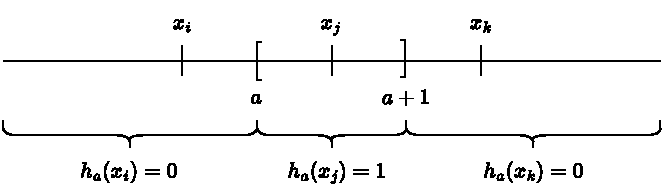
\includegraphics[width=0.75\textwidth]{figures/3_fig1.pdf}
    \caption{}
    \label{fig:3_fig1}
\end{figure}

\noindent\textbf{For 2 points:} all labelings are achievable.

\noindent\textbf{For 3 points:} we will show that the labeling $(1, 0, 1)$ is \textbf{impossible}.

\noindent Let $x_1 < x_2 < x_3$, which implies:
\begin{equation}
\label{eq:1}
x_2 \in [x_1, x_3]
\end{equation}

\noindent The labeling $(1, 0, 1)$ requires:
$$h_a(x_1) = 1, \quad h_a(x_2) = 0, \quad h_a(x_3) = 1$$

\noindent However:
\begin{align*}
\begin{split}
    \left.\begin{array}{l}
        h_a(x_1) = h_a(x_3) = 1 \implies [x_1, x_3] \subseteq [a, a+1] \\[6pt]
        (\ref{eq:1}) \implies x_2 \in [x_1, x_3]
    \end{array}\right\} & \implies x_2 \in [a, a+1] \implies \\
    & \implies h_a(x_2) = 1 \quad \textbf{(contradiction)} 
\end{split}
\end{align*}

\noindent Therefore, $VCdim(\mathcal{H}_1) = 2$.

\subsection*{$\mathrm{VCDim(\mathcal{H}_2)}$}
\addcontentsline{toc}{subsection}{\texorpdfstring{$\mathrm{VCDim(\mathcal{H}_2)}$}{VCDim(H2)}}

\begin{figure}[H]
    \centering
    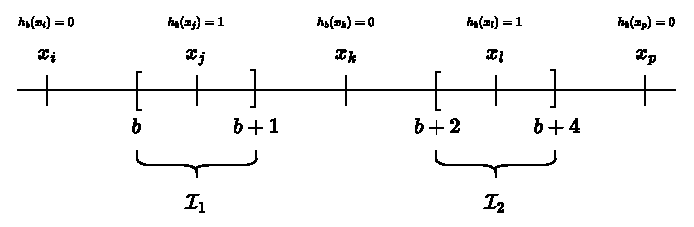
\includegraphics[width=0.75\textwidth]{figures/3_fig2.pdf}
    \caption{}
    \label{fig:3_fig2}
\end{figure}

\noindent\textbf{For 2 points:} all labelings are achievable.

\noindent\textbf{For 3 points:} all labelings are achievable.

\noindent\textbf{For 4 points:}
\newline

\noindent Let $x_1 < x_2 < x_3 < x_4$

\noindent Consider the labeling: $(1, 0, 0, 1)$

\begin{align*}
\begin{split}
    \left.\begin{array}{l}
        h_b(x_1) = h_b(x_4) = 1 \\[6pt]
        h_b(x_2) = h_b(x_3) = 0
    \end{array}\right\} & \implies x_1 \in \mathcal{I}_1 \text{ and } x_4 \in \mathcal{I}_2 \\
    & \implies x_2, \ x_3 \in \big( b+1, \ b+2 \big) \\
    & \implies x_3 - x_1 < 2
\end{split}
\end{align*}

\noindent Consider the labeling: $(1, 0, 1, 0)$

\begin{align*}
\begin{split}
    \left.\begin{array}{l}
        h_b(x_1) = 1 \\[6pt]
        h_b(x_3) = 1 \\[6pt]
        x_3 - x_1 < 2
    \end{array}\right\} & \implies x_1, \ x_3 \in \mathcal{I}_1 \text{ or } x_1, \ x_3 \in \mathcal{I}_2 \\
    & \implies \big[ x_1, \ x_3 \big] \subseteq \mathcal{I}_1 \text{ or } \big[ x_1, \ x_3 \big] \subseteq \mathcal{I}_2
\end{split}
\end{align*}

\noindent However:

\begin{align*}
    x_2 \in \big[ x_1, \ x_3 \big] \implies x_2 \in \mathcal{I}_1 \text{ or } x_2 \in \mathcal{I}_2 \implies h_b(x_2) = 1 \quad \textbf{(contradiction)}
\end{align*}
\newline

\noindent Therefore, $VCdim(\mathcal{H}_2) = 3$.

\subsection*{$\mathrm{VCDim(\mathcal{H}_3)}$}
\addcontentsline{toc}{subsection}{\texorpdfstring{$\mathrm{VCDim(\mathcal{H}_3)}$}{VCDim(H3)}}

\begin{figure}[H]
    \centering
    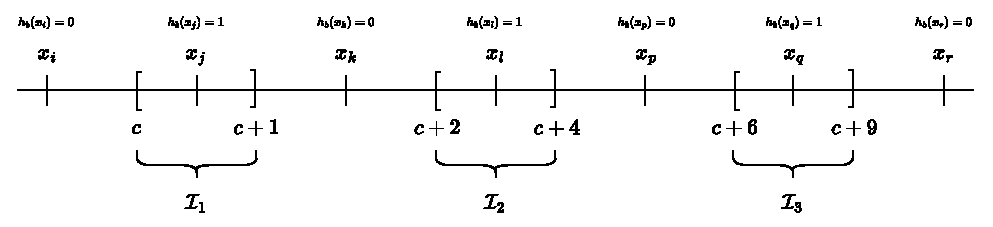
\includegraphics[width=0.75\textwidth]{figures/3_fig3.pdf}
    \caption{}
    \label{fig:3_fig3}
\end{figure}

\noindent\textbf{For 2 points:} all labelings are achievable.

\noindent\textbf{For 3 points:} all labelings are achievable.

\noindent\textbf{For 4 points:} all labelings are achievable.

\noindent\textbf{For 5 points:}
\newline

\noindent Let $x_1 < x_2 < x_3 < x_4 < x_5$

\noindent Consider the labeling $(1, 0, 1, 0, 1)$

\begin{equation}
\label{eq:2}
\begin{split}
    \left.\begin{array}{l}
        x_1 \in \mathcal{I}_1, \ x_3 \in \mathcal{I}_2, \ x_5 \in \mathcal{I}_3 \\[6pt]
        x_2 \in \big( c+1, \ c+2 \big) \\[6pt]
        x_4 \in \big( c+4, \ c+6 \big)
    \end{array}\right\} & \implies x_3 - x_1 > 1 \text{ and } x_5 - x_3 > 2 \implies \\
    & \implies x_5 - x_1 > 3
\end{split}
\end{equation}

\noindent Consider the labeling $(1, 0, 0, 0, 1)$. Note that $x_1$ and $x_5$ cannot lie in the same interval (\ref{eq:2}). 

\noindent \textbf{Case 1: $x_1 \in \mathcal{I}_1,\ x_5 \in \mathcal{I}_2$}

\begin{align*}
\begin{split}
    & x_1 \in \mathcal{I}_1,\ x_5 \in \mathcal{I}_2 \implies x_2,\ x_3,\ x_4 \in \big( c+1,\ c+2 \big) \implies \\
    & \implies x_4 - x_2 < 1,\ x_4 - x_3 < 1,\ x_3 - x_2 < 1
\end{split}
\end{align*}

\noindent \textbf{Case 2: $x_1 \in \mathcal{I}_2,\ x_5 \in \mathcal{I}_3$}

\begin{align*}
\begin{split}
    & x_1 \in \mathcal{I}_2,\ x_5 \in \mathcal{I}_3 \implies x_2,\ x_3,\ x_4 \in \big( c+4,\ c+6 \big) \implies \\
    & \implies x_4 - x_2 < 2,\ x_4 - x_3 < 2,\ x_3 - x_2 < 2
\end{split}
\end{align*}

\noindent \textbf{Case 3: $x_1 \in \mathcal{I}_1,\ x_5 \in \mathcal{I}_3$}

\begin{align*}
\begin{split}
    & x_1 \in \mathcal{I}_1,\ x_5 \in \mathcal{I}_3 \implies x_2,\ x_3,\ x_4 \in \big( c+1,\ c+2 \big) \text{ or } x_2,\ x_3,\ x_4 \in \big( c+4,\ c+6 \big) \\
\end{split}
\end{align*}

\noindent From the Pigeonhole Principle, there exist at least 2 points from $\{x_2,\ x_3,\ x_4\}$ that both lie in either $\big(c+1,\ c+2\big)$ or $\big(c+4,\ c+6\big)$. This implies:
\begin{align*}
    & \exists\ i \in \{2,\ 4\} \text{ s.t.} \quad x_3,\ x_i \text{ both lie in either } \big(c+1,\ c+2\big) \text{ or } \big(c+4,\ c+6\big) \implies \\
    & \implies |x_3 - x_i| < 2
\end{align*}

\noindent However, for the labeling $(1, 0, 1, 0, 1)$, it is impossible for $x_3 \in \mathcal{I}_2$ with $h_c(x_2) = h_c(x_4) = 0$ and $x_3 - x_2 < 2$ and $x_4 - x_3 < 2$.
\newline

\noindent Therefore, $VCdim(\mathcal{H}_3) = 4$.

% --------- Bibliography ---------
\newpage
\printbibliography
\end{document}